\section{绪论}
\subsection{项目背景、发展现状及意义和目标的理解}
变构飞行器能够根据任务需求主动调整外形，是航空航天领域的重要研究方向。本项目旨在利用知识图谱技术对该领域的零散知识进行结构化组织，其核心逻辑可归纳为以下两个方面：

\begin{itemize}[leftmargin=2em, label=\textbullet]
    \item \textbf{行业背景与核心痛点：} 变构飞行器研究涉及气动、结构与控制等多个层面的深度耦合，其多学科交叉特征使得知识获取门槛较高。当前的发展现状表明，核心知识高度分散在海量文献中，存在严重的语义表达不一致和关联关系隐含等痛点，导致研究者在查找和复用知识时需要投入巨大的归纳成本。构建领域知识图谱能够将碎片化的“文献资料”转化为结构化的“知识网络”，从根本上解决知识载体分散与语义检索困难的问题。

    \item \textbf{建设意义与总体目标：} 本项目的研究意义在于通过“规则引擎 + 语义模型”的混合手段，提升专业领域知识获取的可解释性与工程可维护性。项目建设的总体目标是形成一套完整的技术管线：首先构建面向变构飞行器领域的术语与本体体系；其次实现高召回、高精度的实体关系稳定抽取；最后开发可交互的 Web 展示系统，并利用人工金标准对系统性能进行量化验证。通过这一闭环流程，希望实现一套兼顾规范性与工程落地性的领域知识组织原型。
\end{itemize}

\subsection{项目实施技术路线及方案}
本项目总体采用“文献输入—文本预处理—术语构建—知识抽取—图谱导出—系统展示—算法评估”的技术路线。系统以 Python 为核心开发语言，后端基于 FastAPI，前端基于 ECharts，文本处理与统计建模结合 PyMuPDF、pdfminer.six、jieba、pandas 等工具库，并在术语定稿阶段引入 OpenAI 兼容大模型接口。

与单一深度学习方案不同，本项目采用了双模混合智能（Hybrid）架构，即“统计方法 + 规则系统 + LLM 抽取与精筛”。在工程实现上，系统支持检测人工金标词典：当存在人工词典时，维持高标准、高可解释性的规则引擎；否则自动切换为全自动大语言模型模式，以此保证系统的学术可复现性与工程泛化性。此外，大语言模型不仅用于术语归一化和类型定稿，还被深度整合到上下文感知的关系抽取中，并辅以多线程并行调度（ThreadPoolExecutor）以突破调用瓶颈，这既避免了纯规则方法产生的图谱稀疏问题，又显著提升了大规模数据处理的并发效率。

为便于说明系统从原始文献到最终图谱展示的整体演化过程，图~\ref{fig:route} 给出了项目实施技术路线，重点展示了各阶段输入输出之间的衔接关系。读者可以据此把握本项目从数据获取、知识抽取到系统实现的总体流程。

\begin{figure}[H]\centering
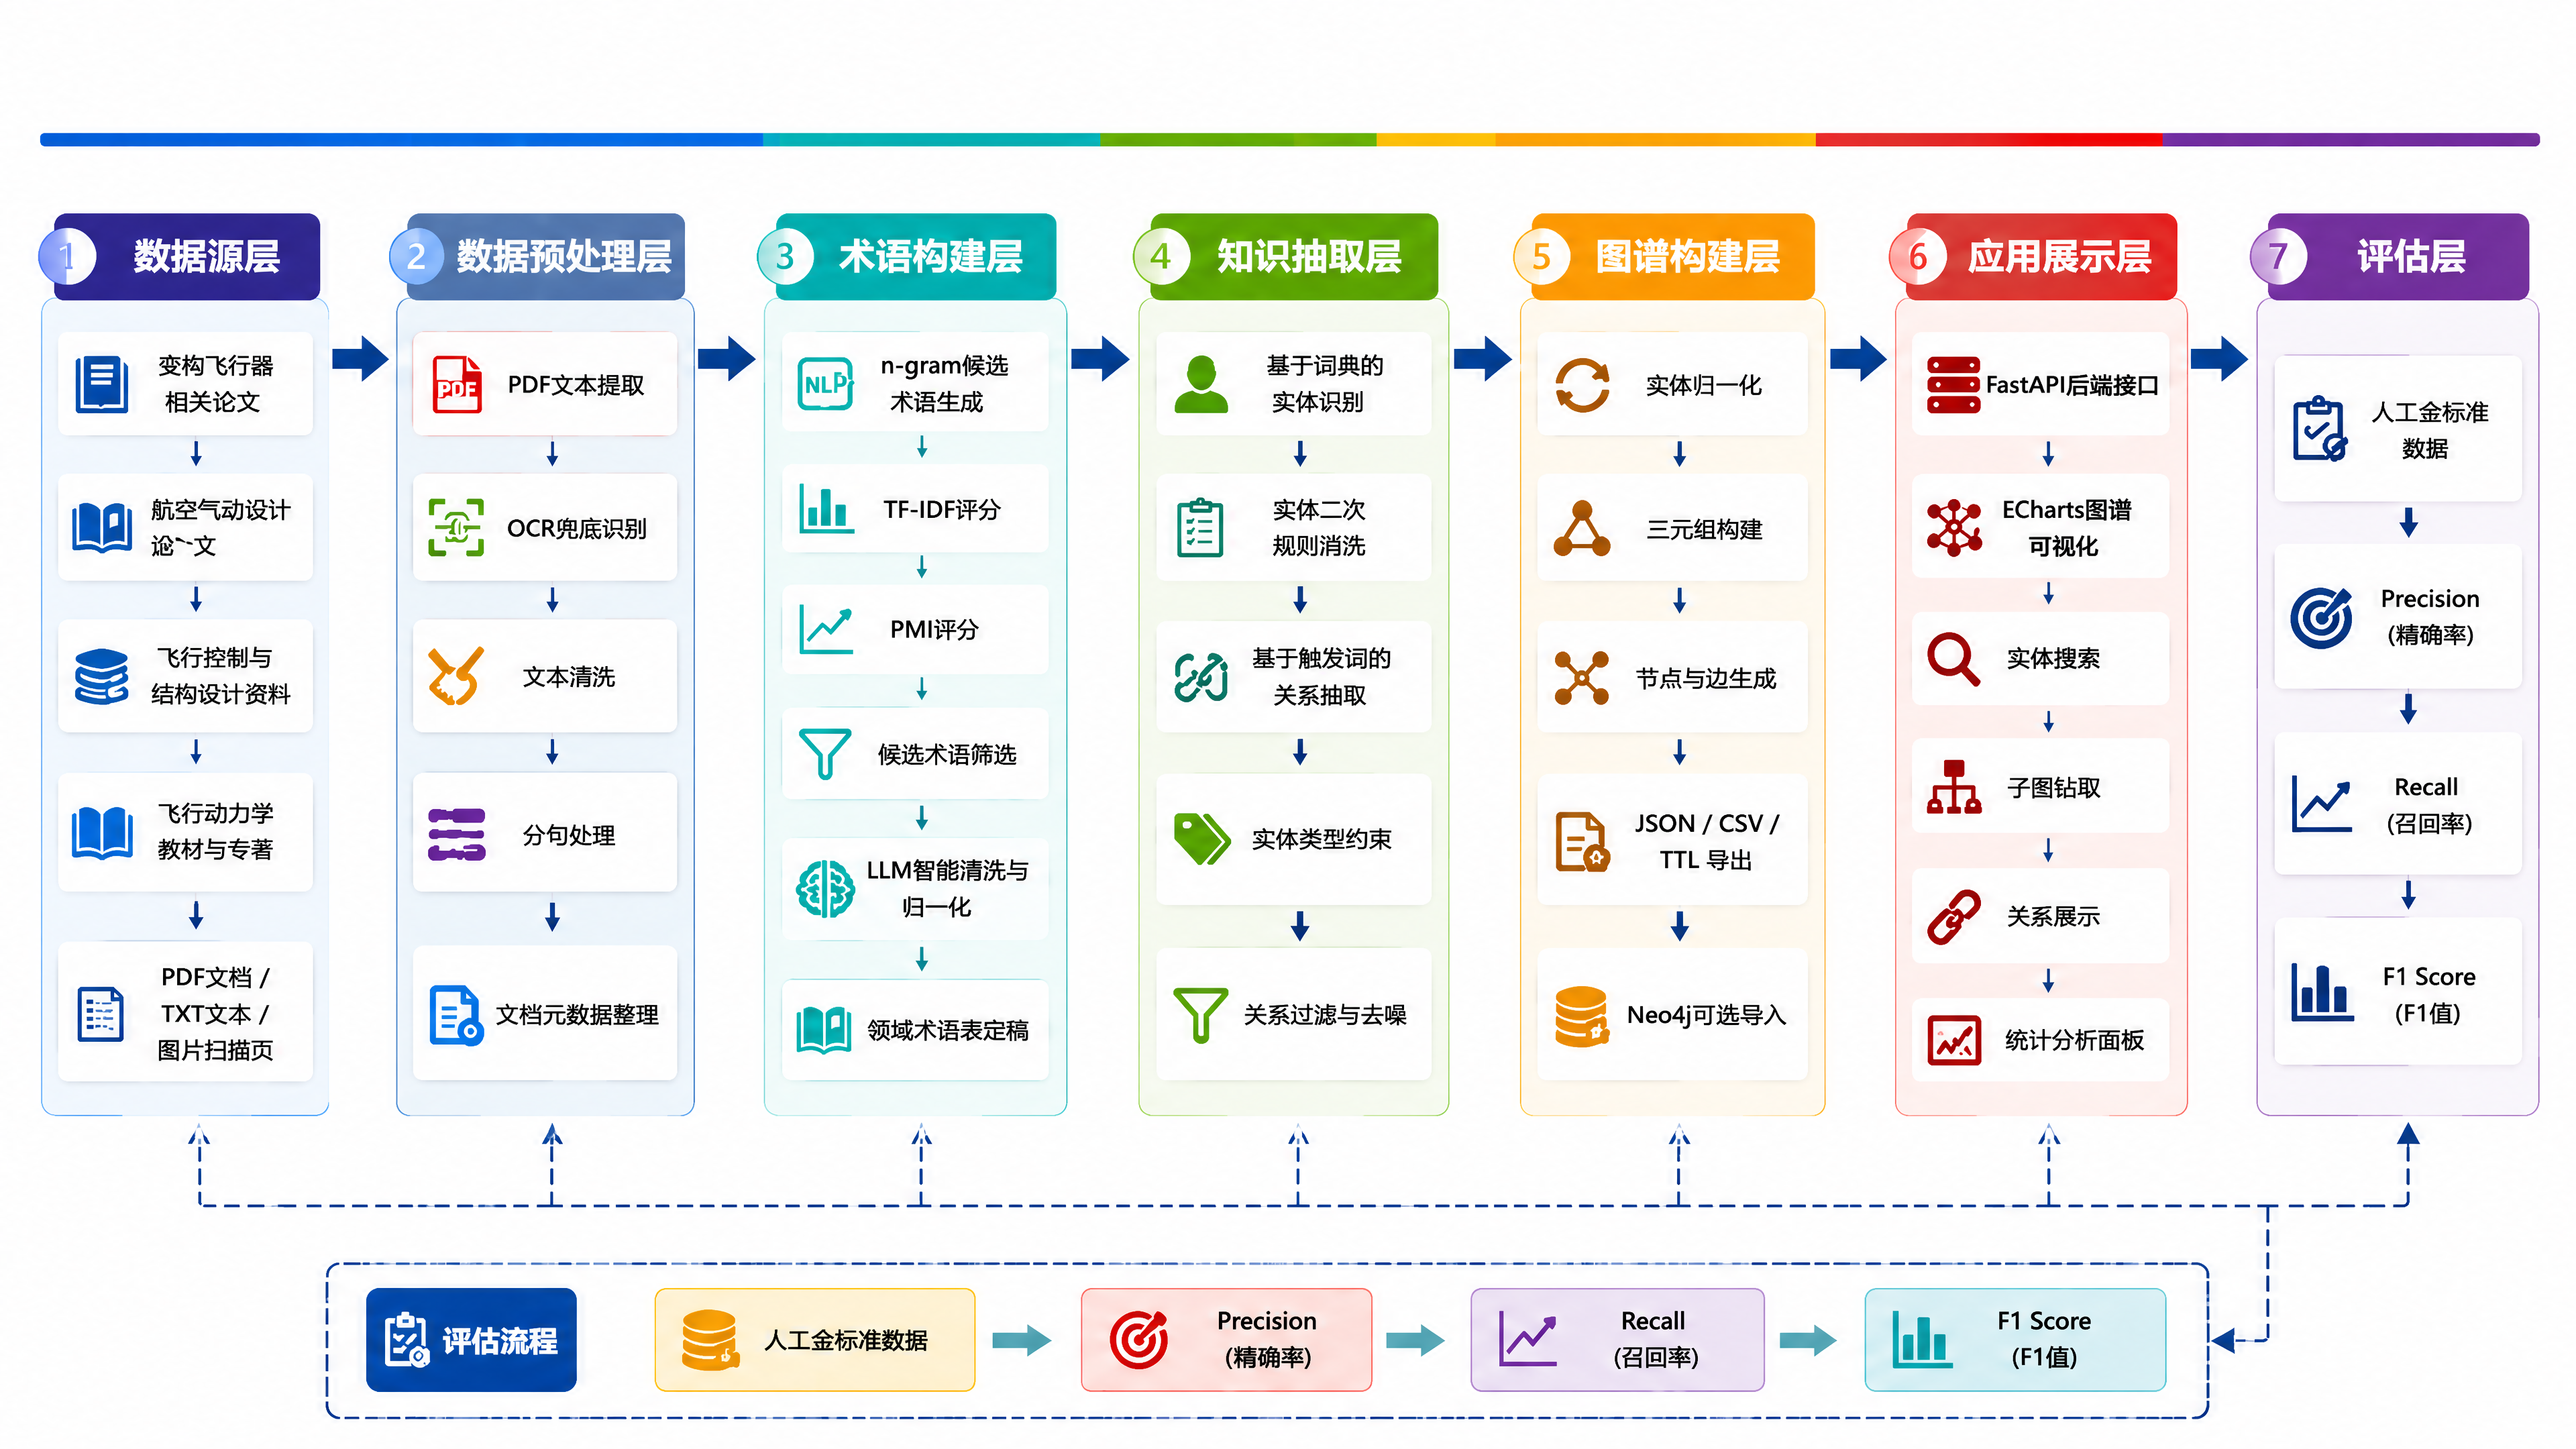
\includegraphics[width=0.90\textwidth]{figures/项目实施技术路线图.png}
\caption{项目实施技术路线图}
\label{fig:route}
\end{figure}

在总体流程明确之后，还需要进一步说明系统内部各模块的组织方式。图~\ref{fig:arch} 展示了系统总体架构，从数据层、处理层、抽取层到图谱层、服务层和展示层逐层展开，体现了本项目模块化、分层化的工程组织思路。

\begin{figure}[H]\centering
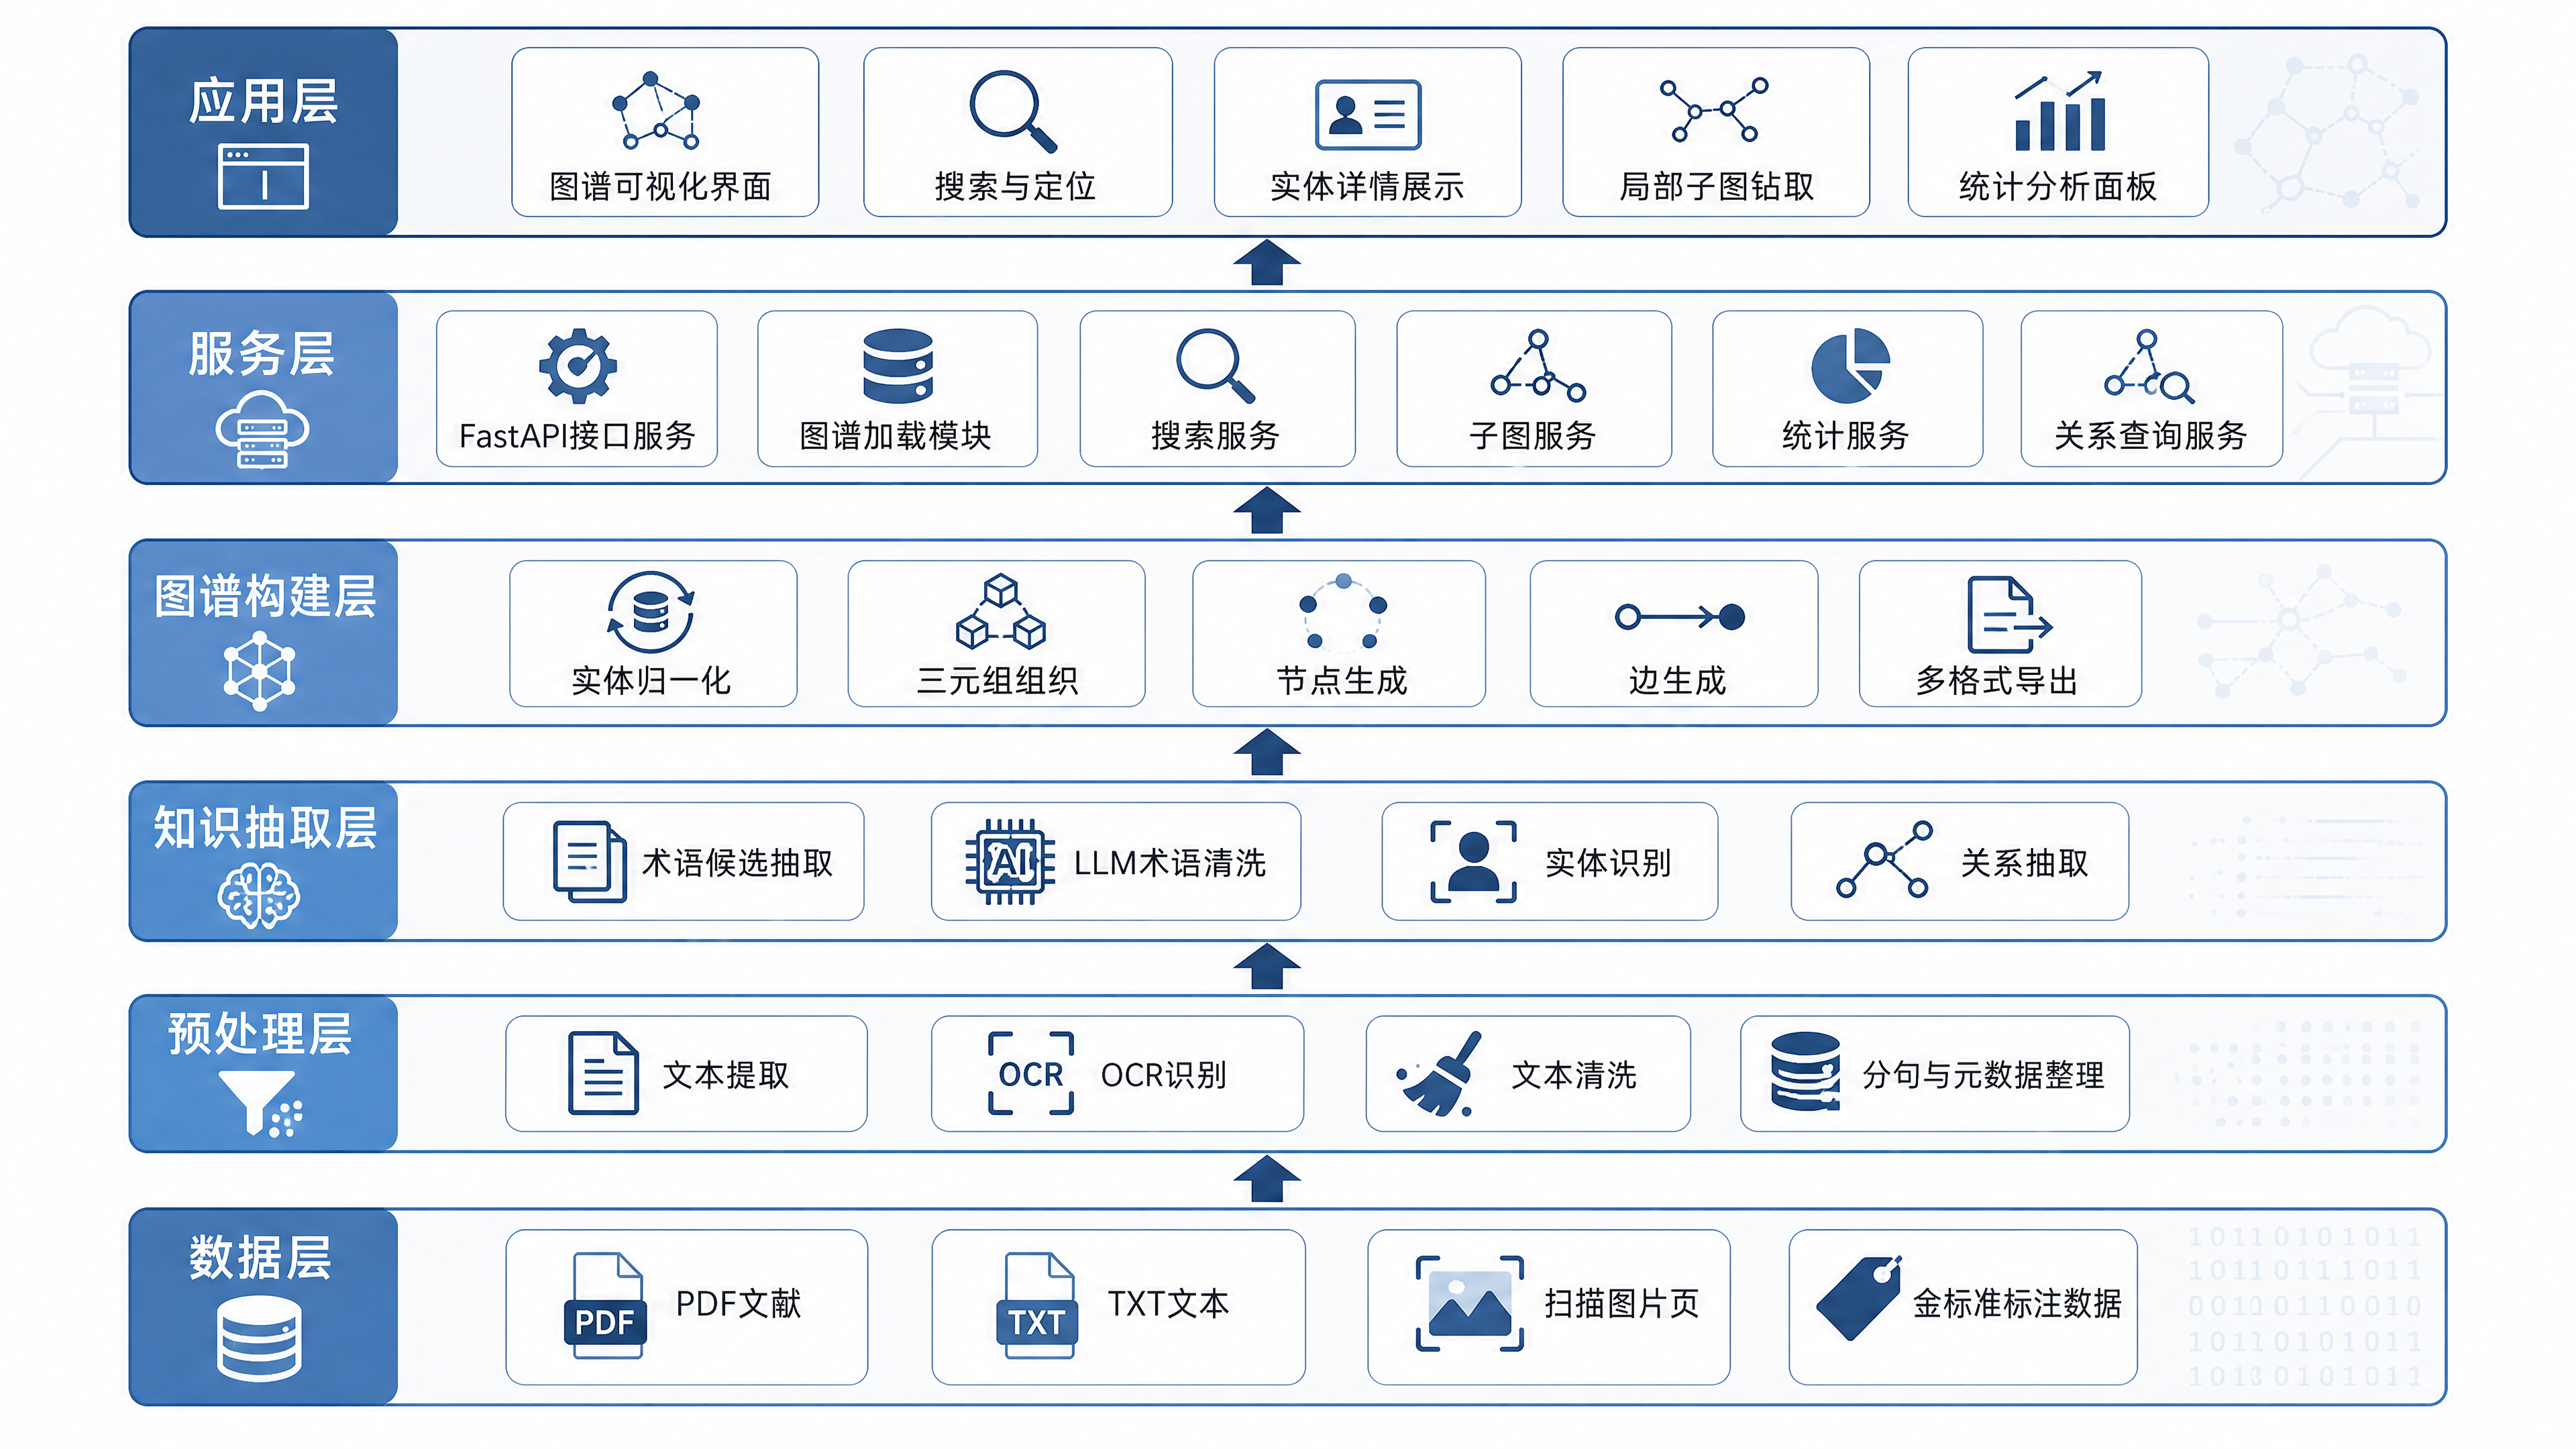
\includegraphics[width=0.86\textwidth]{figures/系统总体架构图.png}
\caption{系统总体架构图}
\label{fig:arch}
\end{figure}
